% =========================================================================
% 《高中數學實驗教材》第一冊（高一上） 
% 第三章 數的概念
% =========================================================================

\section{數的概念}\label{sec:ch3}

「自然數系」、「有理數系」和「實數系」，這些「數」是由種種自然界所常見的「量」，歸納其共同性質而得的體系。它們是有效討論各種關於量的問題所不可或缺的工具。上述諸數系的基本性質是數學的基礎與根源所在。本章將詳述數的源起，自然數及有理數的基本性質。由於實數系的一部份性質較為深些，而且在目前並不需要用它，故實數系的基本性質，將留待第二冊才為同學們作一有系統的介紹。

\subsection{數的源起}\label{sec:3-1}

在第一章的甲段討論數學的題材時，我們已簡略地談到數的源起。對於具有天然個別單元的量，我們只需要「數一數」它們有多少「個」，而自然數也就是用以「計數」個數的工具。同學們都已熟習自然數的加與乘這兩種基本運算，在下一節中我們將詳述自然數系對於加與乘這兩種基本運算所具有的基本性質。現在讓我們簡要地談談加與乘這兩種運算的源起：

\subsubsection*{甲、「1」是自然的起點}\label{subsec:plus_one}

「1」是自然的起點，
\begin{equation*}
  2=1+1, \quad 3=2+1, \quad 4=3+1, \quad 5=4+1, \quad \dots, \quad 97=96+1, \quad \dots
\end{equation*}
所以「$+1$」（加一）是自然中最原始的運算。

事實上，我們所知道的加法與乘法，通通可以看做是「$+1$」這個運算的推廣，下面我們繼續說明這件事。

假如我們把「$+1$」這種運算做兩遍，如 $(5+1)+1=5+2$，或 $(6+1)+1=6+2$ 等，這就是「$+2$」的意思\footnote{「$(a+1)+1$」這個符號，就是表示把「$a$」這個數，用「$+1$」連做兩遍的意思。小括弧 $(a+1)$ 表示做第一次「$+1$」；做完之後，再「$+1$」一次，豈不是剛好做了兩遍？因此，適當地利用符號，可以將一些要用文字才能說清楚的事，說得更明白。}，亦即
\begin{equation*}
  a+2 \text{ 的意思是 } (a+1)+1
\end{equation*}
以此類推，「$+3$」就是把「$+1$」重複做三遍，「$+4$」就是把「$+1$」重複做四遍……等等，亦即
\begin{align*}
  a+3 &= ((a+1)+1)+1 \\
  a+4 &= (((a+1)+1)+1)+1
\end{align*}
所以「$a+b$」就是對 $a$ 作 $b$ 次「$+1$」運算的縮寫。

其次讓我們看一看乘法的運算：
\begin{align*}
  a &= 1 \times a, \\
  a+a &= 2 \times a, \\
  a+a+a &= 3 \times a, \\
  a+a+a+a &= 4 \times a,
\end{align*}
上面諸式，不難看出 $b \times a$ 也就是 $b$ 個 $a$ 相加的縮寫。

\subsubsection*{乙、度量與數系的擴張}\label{subsec:measure_expansion}

在第一章的甲段中，我們也談到另一類不具有「天然單元」的量，如「長度」、「質量」、「體積」等，並以長度為例，討論了如何去度量這一類的量。簡單的說，度量的方法是先取一個人為的單位，然後去求「所要度量的量」和「所取定的單位」間的比值，這種比值是一個「實數」，換言之，「實數系」也是度量的工具。從對長度的度量的討論中，有
\begin{equation*}
  \text{實數系} \supset \text{有理數系} \supset \text{自然數系}
\end{equation*}
這一重要的相互關係。我們將循序漸進，先去瞭解「自然數系」的性質，然後經由「自然數系」和「有理數系」間的相互關係去瞭解「有理數系」的性質。在第二冊中，我們將再進一步經由「有理數系」和「實數系」間的相互關係去瞭解「實數系」的性質。

\subsection{自然數系的基本性質}\label{sec:3-2}

「數」是討論種種「關於量的問題」的有效工具，但是我們必須先切實瞭解這些「工具」的基本特性才能真正發揮其效用。自然數系是上述「數」中最簡單也是最基本的，所以自然數系的基本性質是整個體系的重要基礎！同學們切不可因為「它們看起來簡單平凡」而忽略它，要知道世間有用的道理就是那些簡單而不凡的道理，要點在於：能心領神會、能活用這些簡單而不凡的道理！

\subsubsection*{甲、本節符號的用法}\label{subsec:nat_notation}

我們將用 $\mathbb{N}$ 表示所有自然數所成的集合，即
\begin{equation*}
  \mathbb{N} = \{1, 2, 3, 4, \dots, n, \dots\}
\end{equation*}
我們將用小寫字母 $a, b, c, \dots$ 等來表示 $\mathbb{N}$ 中的任何一個元素。於是，我們就可以用這樣的符號，很方便地去討論，去描述自然數系的「通性」。譬如：
\begin{equation*}
  a+b \neq 1
\end{equation*}
表示任何兩個自然數的和絕不等於 $1$。換言之，上述一個式子充分地表達了所有下述式子的全體：（注意：零「$0$」不屬於 $\mathbb{N}$。）
\begin{align*}
  1+1 \neq 1, \quad 1+2 \neq 1, \quad 1+3 \neq 1, \quad 1+4 \neq 1, \quad \dots \\
  2+1 \neq 1, \quad 2+2 \neq 1, \quad 2+3 \neq 1, \quad 2+4 \neq 1, \quad \dots \\
  3+1 \neq 1, \quad 3+2 \neq 1, \quad 3+3 \neq 1, \quad 3+4 \neq 1, \quad \dots \\
  4+1 \neq 1, \quad 4+2 \neq 1, \quad 4+3 \neq 1, \quad 4+4 \neq 1, \quad \dots
\end{align*}
同理，下述諸式：
\begin{align*}
  1+1 = 1+1, \quad 1+2 = 2+1, \quad 1+3 = 3+1, \quad 1+4 = 4+1, \quad 1+5 = 5+1, \quad \dots \\
  2+2 = 2+2, \quad 2+3 = 3+2, \quad 2+4 = 4+2, \quad 2+5 = 5+2, \quad \dots \\
  3+3 = 3+3, \quad 3+4 = 4+3, \quad 3+5 = 5+3, \quad \dots
\end{align*}
就可以簡潔地用 $a+b = b+a$ 總括地加以表達。

\subsubsection*{乙、自然數系基本性質}\label{subsec:nat_axioms}

列述自然數系的基本性質如下：
\begin{enumerate}[I.]
  \item 任何一自然數，均可由 $1$ 開始，經有限次「$+1$」運算而得。換句話說，由 $1$ 開始，逐次「$+1$」，即可得到任一自然數，這就叫做「\textbf{數學歸納法（mathematical induction）原理}」。
  \item $(a+b)+c = a+(b+c)$。（加法結合律）
  \item $a+b = b+a$。（加法交換律）
  \item $a+b = c+b \iff a = c$。（$\Rightarrow$ 的部分叫做加法對消律）
  \item $(a+b) \cdot c = a \cdot c + b \cdot c$。（分配律）
  \item $a \cdot b = b \cdot a$。（乘法交換律）
  \item $(a \cdot b) \cdot c = a \cdot (b \cdot c)$。（乘法結合律）
  \item $a \cdot b = c \cdot b \iff a = c$。（$\Rightarrow$ 的部分叫做乘法對消律）\\
  （注意：零「$0$」不是自然數，所以 $b \neq 0$。）
\end{enumerate}

同學們對於自然數的次序都已十分清楚，現在我們來仔細看看甚麼叫做 $3 < 5$。我們知道 $3 < 5$，是因為 $5$ 在自然數中，排在 $3$ 的後面。換句話說，由 $3$ 開始，作兩次「$+1$」運算便得到 $5$，即 $3+2=5$。一般地說，設 $a, b$ 都是自然數，如果有一個自然數 $u$，使得 $a+u=b$，我們就說 $a$ 小於 $b$，記做 $a < b$；或者說 $b$ 大於 $a$，記做 $b > a$。

\subsection*{習題 3-1}\label{sec:ex3-1}
\addcontentsline{toc}{subsection}{習題 3-1}

\begin{enumerate}[1., leftmargin=2em]
  \item 求下列各組數相除的商數與餘數：
  \begin{enumerate}[(i)]
    \item $a = 732, \quad b = 24$。
    \item $a = 365, \quad b = 7$。
    \item $a = 719415, \quad b = 365$。
    \item $a = 30, \quad b = 7$。
    \item $a = 1973, \quad b = 54$。
  \end{enumerate}
  \item 一數 $x$ 除以 $7$，餘 $3$；一數 $y$ 除以 $7$，餘 $2$；那麼 $xy$ 除以 $7$ 的餘數是多少呢？
  \item 一數 $x$ 除以 $9$，餘 $4$；一數 $y$ 除以 $9$，餘 $5$；求 $xy$ 除以 $9$ 的餘數。
\end{enumerate}

\subsubsection*{丙、數學歸納法}\label{subsec:induction}

我們現在來略為討論一下數學歸納法，數學歸納法是自然數的性質 I 的另一種表示方法，有用處的地方很多，我們今後也會常常用到。現在我們舉例說明如下：

\noindent{\textbf{【例 1】}}求證
\begin{equation}\label{eq:sum_integers_formula}
  1+2+3+\dots+n = \frac{n(n+1)}{2} \qquad \dots\dots (1)
\end{equation}

\noindent{\textbf{【證明】}}當 $n=1$ 時，我們有
\begin{equation*}
  1 = \frac{1(1+1)}{2}
\end{equation*}
因此 (1) 是對的，我們也不難看出在 $n=2, 3, 4$ 時 (1) 式都滿足，但是，我們怎樣才知道 (1) 式是對所有的自然數都對呢？

我們想一想，甚麼叫「所有的自然數」，又，我們怎樣才能得到「所有的自然數」？根據性質 I，所有的自然數可以自 $1$ 開始，一次一次地由「$+1$」而得到，因此，我們來看一看怎樣利用這個性質來證明 (1)。

在 $n=k$ 時，(1) 成為
\begin{equation}\label{eq:ind_step_k}
  1+2+\dots+k = \frac{k(k+1)}{2} \qquad \dots\dots (2)
\end{equation}
在 $n=k+1$ 時，(1) 的左邊應該是
\begin{equation}\label{eq:ind_step_lhs}
  1+2+\dots+k+(k+1) \qquad \dots\dots (3)
\end{equation}
右邊應該是
\begin{equation}\label{eq:ind_step_rhs}
  \frac{(k+1)(k+2)}{2} \qquad \dots\dots (4)
\end{equation}
（我們還不知道 (2) 是否成立，也不知道 (3) 是否等於 (4)）但是假如我們：
\begin{align*}
  &\text{從 } n=1 \text{ 證到 } n=2 (=1+1) \\
  &\text{從 } n=2 \text{ 證到 } n=3 (=2+1) \\
  &\text{從 } n=3 \text{ 證到 } n=4 (=3+1) \\
  &\dots\dots \\
  &\text{從 } n=k \text{ 證到 } n=k+1 \qquad \dots\dots (5)
\end{align*}
那麼，我們豈不是對「所有的自然數」都證明了 (1)？請注意在這裏 $k$ 是一個典型的自然數。因此，如果我們證明了 $(2) \implies (3)=(4)$，那麼便等於證明了 (5) 的全體。所以，若是要對所有的自然數證明 (1) 式，我們只要再證明 $(2) \implies (3)=(4)$ 就夠了，這就是數學歸納法的精神。

根據
\begin{align*}
  (3) &= 1 + 2 + \dots + k + (k+1) \\
  &= (1 + 2 + \dots + k) + (k+1) \\
  &= \frac{k(k+1)}{2} + (k+1) \\
  &= (k+1)\left(\frac{k}{2} + 1\right) \\
  &= (k+1)\frac{k+2}{2} \\
  &= \frac{1}{2}(k+1)(k+2) = (4)
\end{align*}
因此，我們用數學歸納法證明了 (1)。

有些不等式也可以用數學歸納法證明，讓我們舉一個例子來說明：

\noindent{\textbf{【例 2】}}設 $p > 0$，求證 $(1+p)^n \ge 1+np$，式中 $n$ 為自然數。

\noindent{\textbf{【證明】}}當 $n=1$ 時，上式的左右兩邊都是 $1+p$。所以不等式成立，而實際上這時可以改成等號。

設 $(1+p)^k \ge 1+kp$，則
\begin{align*}
  (1+p)^{k+1} &= (1+p)^k (1+p) \ge (1+kp)(1+p) \\
  &= 1 + kp + p + kp^2 = 1 + (k+1)p + kp^2 > 1 + (k+1)p.
\end{align*}
因此不等式對 $n=k+1$ 亦成立。故由數學歸納法知，對所有的自然數 $n$，不等式皆成立。

在運用數學歸納法時，必須注意其步驟的有效性。例如有人提出：若任意給定 $n$ 點，求證皆在同一直線上。其錯誤在於由 $k=2$ 到 $k=3$ 時兩子集的交集不足以決定唯一直線。我們應該把題目改成：若任意三點皆在一直線上，則任意 $n$ 點必在一直線上。

\subsection*{習題 3-2}\label{sec:ex3-2}
\addcontentsline{toc}{subsection}{習題 3-2}

\begin{enumerate}[1., leftmargin=2em]
  \item 有人用下法證明全世界的人性別都一樣。設一集合 $M_n$ 包含 $n$ 個人，則想證明 $M_n$ 中的人性別都一樣。當 $n=1$ 時，$M_n$ 中只有一個人，當然其性別是唯一的。現在假定命題 $n=k$ 時成立；再假定 $M_{k+1}$ 是包含 $k+1$ 個人的集合，在 $M_{k+1}$ 中選定兩個人 $x$ 和 $y$，則 $M_{k+1} \setminus \{x\}$ 和 $M_{k+1} \setminus \{y\}$ 都是只包含 $k$ 個人的集合，所以其中的人性別都一樣，因而 $x, y$ 和 $M_{k+1} \setminus \{x, y\}$ 中任何人的性別都相同，故 $M_{k+1}$ 中諸位的性別必全相同。請指正這證明錯在哪裡？
  \item 等差級數求和的公式也可以用數學歸納法證明，你能做出嗎？
  \item $n \in \mathbb{N}$，試說明 $n^2 - n + 41$ 不為質數。
  \item 試用數學歸納法證明下式：
  \begin{equation*}
    1^2 + 2^2 + 3^2 + \dots + n^2 = \frac{1}{6}n(n+1)(2n+1).
  \end{equation*}
  \item 設 $n$ 為正整數，試證
  \begin{equation*}
    (1^5 + 2^5 + 3^5 + \dots + n^5) + (1^7 + 2^7 + 3^7 + \dots + n^7) = 2 \left[\frac{n(n+1)}{2}\right]^4.
  \end{equation*}
  \item $1^3 + 2^3 + 3^3 + \dots + n^3 = (1+2+3+\dots+n)^2$.
  \item 設 $n$ 是正整數，試證 $1 + 3 + 5 + \dots + (2n-1) = n^2$。
  \item $1 \cdot 2 \cdot 3 + 2 \cdot 3 \cdot 4 + \dots + n(n+1)(n+2) = \frac{1}{4}n(n+1)(n+2)(n+3)$。
\end{enumerate}

\subsubsection*{丁、基本性質的推論}\label{subsec:nat_corollaries}

利用上述「自然數系」的基本性質 I--VIII，我們可以推演得所有「自然數系」的重要性質，而且以後我們逐步討論整數系，有理數系及實數系等數系的基本性質時，上述自然數系的基本性質 I--VIII 就是我們的起點。

我們現在列舉幾個基本性質的簡單推論：

\noindent{\textbf{XI.}}
\begin{enumerate}[(1)]
  \item $a > b \iff a+c > b+c$.
  \item $a = b \iff a+c = b+c$.
  \item $a < b \iff a+c < b+c$.
\end{enumerate}

\noindent{\textbf{【證明】}}$a > b \iff$「存在 $u \in \mathbb{N}$，使得 $a=b+u$」（“$>$”的定義）
\begin{align*}
  &\iff a+c = (b+u)+c \\
  &\iff a+c = b+(u+c) && \text{(II)} \\
  &\iff a+c = b+(c+u) && \text{(III)} \\
  &\iff a+c = (b+c)+u && \text{(II)} \\
  &\iff a+c > b+c && \text{(“$>$”的定義)}
\end{align*}
同理可知 $a < b \iff a+c < b+c$。

\noindent\textbf{註}：往後證明或運算時，當然不必如上面這樣細項，譬如從 $a+c=(b+u)+c$ 我們可以把上述三步合成一步，導得 $a+c=(b+c)+u$。

\medskip
\noindent{\textbf{XII.}}
\begin{enumerate}[(1)]
  \item $a > b \iff a \cdot c > b \cdot c$.
  \item $a = b \iff a \cdot c = b \cdot c$.
  \item $a < b \iff a \cdot c < b \cdot c$.
\end{enumerate}
（注意：$c \in \mathbb{N}$ 所以 $c$ 是正的！）

\noindent{\textbf{【證明】}}：我們現在先證明 (1)
\begin{align*}
  a > b &\implies \text{「存在 } u \in \mathbb{N} \text{ 使得 } a=b+u\text{」} && \text{(“$>$”之定義)} \\
  &\implies a \cdot c = (b+u) \cdot c = bc + uc && \text{(V)} \\
  &\implies a \cdot c > bc. && \text{(“$>$”之定義)}
\end{align*}
反之，若 $ac > bc$，我們想證明 $a > b$，因 $a > b$，$a = b$，$a < b$ 只有一種，必有一種會成立，所以我們先看 $a < b$ 會不會成立。

假如 $a < b$，則 $b > a$，而由上面的證明可知 $bc > ac$，或 $ac < bc$，但是我們假定 $ac > bc$，所以，$a < b$ 不會成立。

再看 $a = b$ 會不會成立呢？由 VIII，可知 $a = b \implies ac = bc$，又和我們的假定 $ac > bc$ 矛盾，因此 $a = b$ 也不會成立。因此只有 $a > b$ 會成立，至此我們證明了 (1)。

在 (1) 的敘述中 $a, b$ 互換，便得到 $b > a \iff bc > ac$，亦即 $a < b \iff ac < bc$。

\noindent\textbf{註}：上面最後所用的證明方法，叫做\textbf{窮舉法}。

\noindent\textbf{注意}：當問題的本身有相當的對稱性時，適當地利用這些對稱性有時可以省去很多不必要的麻煩，請注意我們怎樣利用題目中已證明的結果，也請注意我們為什麼在 (3) 的證明裏可以簡單地說「與 $b$ 交換」，這是因為 $a$ 和 $b$ 都是任意自然數的緣故。XII 中的敘述，事實上可以用 $a > b \iff ac > bc$ 來表示，請問我們為甚麼可以省去了 $a < b \iff ac < bc$ 這一部分？請問，我們這樣做時，有沒有損及這敘述的一般性？

\medskip
\noindent{\textbf{X.}} 如果 $a > b$，並且 $b > c$，則 $a > c$。

\noindent{\textbf{【證明】}}「$a > b$」和「$b > c$」$\implies$「存在 $u \in \mathbb{N}$，使 $a=b+u$」和「存在 $u' \in \mathbb{N}$，使 $b=c+u'$」（“$>$”的定義）。
\begin{align*}
  a &= b+u = (c+u')+u = c+(u'+u) && \text{(II)} \\
  &\implies a > c. && \text{(“$>$”的定義)}
\end{align*}

\medskip
\noindent{\textbf{(XI')}} 如果 $a > b$ 並且 $c > d$，則 $a+c > b+d$。

\medskip
\noindent{\textbf{(XII')}} 如果 $a > b$ 並且 $c > d$，則 $a \cdot c > b \cdot d$。

\medskip
\noindent{\textbf{【例 1】}}對於任何自然數 $a$、$b$、$n$，如果 $a > b$，那麼 $a^n > b^n$。

\noindent{\textbf{【證明】}}我們利用歸納法來證明：

當 $n=1$ 時，$a > b$ 成立。

設 $n=k$ 時，$a^k > b^k$ 成立，由於性質 XII' 和 $a > b$ 的性質，我們有 $a^{k+1} > b^{k+1}$，所以對於任何 $n$，這個式子都成立。

\subsection*{習題 3-3}\label{sec:ex3-3}
\addcontentsline{toc}{subsection}{習題 3-3}

\begin{enumerate}[1., leftmargin=2em]
  \item 試證明上面的性質 (XI') 及 (XII')。
  \item 試證 $2^{10n} > 3^{2n}$，$n$ 為自然數。
  \item 試證 $2^{3n} < 10^n$，$n$ 為自然數。
  \item 利用 $5^2 = 3^2 + 4^2$，證明 $5^n > 3^n + 4^n$，$n > 2$。
  \item 當 $n \ge 4$ 時，證明 $3^n > n^3$。〔提示：$(n+1)^3 = n^3 + 3n^2 + 3n + 1$〕
\end{enumerate}

\subsubsection*{戊、數系性質的初步應用}\label{subsec:nat_app}

學到這裏，許多同學可能會有些「吃悶葫蘆」的感覺，因為我們一直在吹這些如分配律、交換律、結合律、對消律，………等數系基本性質多麼要緊，多麼有用，但是它們的要緊性，它們的用處到底在什麼地方呢？我們在這裏先講一個小故事，初步說明一下它們的廣泛應用。

\noindent{\textbf{【例 1】}}「等差級數」的求和：

據說當年大數學家高斯（C. F. Gauss 1777～1855）在六、七歲時就是老愛發問，有一次老師給他下面的題目，叫他好好去算，希望他能夠安靜一會兒，題目是：
\begin{equation*}
  1+2+3+4+5+\dots+96+97+98+99+100 = ?
\end{equation*}
殊不知不到一、兩分鐘，高斯小朋友就迅速而準確地把上面一百個數目加好了，他的算法如下：（你說呢？）
\begin{align*}
  & 1 + 2 + 3 + \dots + 98 + 99 + 100 \\
  +) \quad & 100 + 99 + 98 + \dots + 3 + 2 + 1 \\
  \hline
  & 101 + 101 + 101 + \dots + 101 + 101 + 101 \quad (\text{共 } 100 \text{ 個}) \\
  &= 100 \times 101.
\end{align*}
所以
\begin{align*}
  1+2+3+\dots+98+99+100 &= \frac{1}{2} \times 100 \times 101 \\
  &= 5050.
\end{align*}
他的老師對他這麼小小年紀，即能靈活運用數的性質去解決問題，大為賞識器重。

上述算法也就是「等差級數」的求和法；下列級數叫做「等差級數」，
\begin{equation*}
  a+(a+d)+(a+2d)+\dots+(a+(n-1)d)
\end{equation*}
$a$ 叫做它的首項，$d$ 叫做它的公差，$n$ 是它的項數，令 $S$ 為其總和，則由下式
\begin{align*}
  & a + (a+d) + (a+2d) + \dots + (a+(n-1)d) = S \\
  +) \quad & (a+(n-1)d) + (a+(n-2)d) + \dots + a = S \\
  \hline
  & (2a+(n-1)d) + (2a+(n-1)d) + \dots + (2a+(n-1)d) = 2S \\
  &= n(2a+(n-1)d)
\end{align*}
故
\begin{align*}
  S &= \frac{n}{2}(2a+(n-1)d) \\
  &= \frac{\text{項數}(\text{首項}+\text{末項})}{2}
\end{align*}

講到等差級數可以順便提一下等比級數：
\begin{equation*}
  a+(a \cdot r)+(a \cdot r^2)+\dots+(a \cdot r^{n-1})
\end{equation*}
其中 $a$ 稱為首項，$r$ 稱為公比，$n$ 是項數，令 $S$ 為總和，則由下式
\begin{align*}
  & a + ar + ar^2 + \dots + ar^{n-1} = S \\
  -) \quad & ar + ar^2 + \dots + ar^{n-1} + ar^n = rS \\
  \hline
  & a - ar^n = S - rS
\end{align*}
即 $S(1-r) = a - ar^n$，可得
\begin{equation*}
  S = \frac{a - ar^n}{1-r}
\end{equation*}

以上求法有它巧妙整齊的技巧，與等差級數求和的方法類似，但我們亦可以從另一角度來看這問題，這就是下一例題所要用的遞迴證法。

\medskip
\noindent{\textbf{【例 2】}}求證 $1+2+4+8+\dots+2^{n-1} = 2^n - 1$。

\noindent{\textbf{【證明】}}（請在各推論的後面上理由）。

我們只要證明：
\begin{equation*}
  1+1+2+4+\dots+2^{n-1} = 2^n \qquad \dots\dots (1)
\end{equation*}
就好。(1) 式的左邊
\begin{align*}
  &= 1+1+2+2^2+2^3+\dots+2^{n-1} \\
  &= (1+1)+2+2^2+2^3+\dots+2^{n-1} \\
  &= 2+2+2^2+\dots+2^{n-1} \\
  &= 2^2+2^2+2^3+\dots+2^{n-1} \\
  &= 2^3+2^3+\dots+2^{n-1} \\
  &= \dots\dots \\
  &= 2^{n-1}+2^{n-1} \\
  &= 2^n.
\end{align*}
用例 2 的聚項求和法可以推廣到等比級數求和公式，推廣的步驟留作習題，至於數列與級數則留待適當的時候介紹，目前不必花許多時間鑽研。

以上的例子，有一個有趣的解釋。假如你跟別人賭博，第一次下注 $1$ 元，如果輸了，便下注 $2$ 元，如果再輸了，便下注 $2^2=4$ 元，再輸了便下注 $2^3=8$ 元，……直到你贏一次為止，假如你一直輸了 $n$ 次，而在第 $n+1$ 次才贏，那麼你贏回的錢是
\begin{equation*}
  2^n - (1+2+4+\dots+2^{n-1}) = 1.
\end{equation*}
因此，看起來似乎是：「假如你不停的賭下去，每次賭注加倍，只要贏一次，那麼，我一定會贏一塊錢。」

這也許就是為什麼許多賭徒傾家蕩產的理由。進一步的理由，等到高三或然率的時候，可以清楚地向各位同學說明。在這裏，我們只提醒一句：在我們想到「贏一塊錢」的時候，我們還要同時考慮「贏一塊錢的機會」，在另一方面，我們也要提醒大家，在 $n$ 並不很大時，這個數目 $2^n$ 會變得非常大，例如

\begin{table}[htbp]
\centering
\small
\renewcommand{\arraystretch}{1.2}
\begin{tabular}{|c|l|l|}
\hline
$n$ & \multicolumn{1}{c|}{第 $n$ 次下注額} & \multicolumn{1}{c|}{連輸 $n$ 次後輸的總數} \\ \hline
1  & $1 = 2^0$      & $1$ \\ \hline
2  & $2 = 2^1$      & $1+2 = 3$ \\ \hline
3  & $4 = 2^2$      & $1+2+4 = 7$ \\ \hline
4  & $8 = 2^3$      & $1+2+4+8 = 15$ \\ \hline
5  & $16 = 2^4$     & $1+2+\dots+16 = 31$ \\ \hline
6  & $32 = 2^5$     & $1+2+\dots+32 = 63$ \\ \hline
7  & $64 = 2^6$     & $1+2+\dots+64 = 127$ \\ \hline
8  & $128 = 2^7$    & $255$ \\ \hline
9  & $256 = 2^8$    & $511$ \\ \hline
10 & $512 = 2^9$    & $1023$ \\ \hline
11 & $1024 = 2^{10}$ & $2047$ \\ \hline
12 & $2048 = 2^{11}$ & $4095$ \\ \hline
13 & $4096 = 2^{12}$ & $8191$ \\ \hline
14 & $8192 = 2^{13}$ & $1+2+\dots+8192 = \frac{2^{14}-1}{2-1} = 16384-1$ \\ \hline
15 & $16384 = 2^{14}$ & $1+2+\dots+16384 = \frac{2^{15}-1}{2-1} = 32768-1$ \\ \hline
16 & $32768 = 2^{15}$ & \\ \hline
\end{tabular}
\end{table}

因此，假如你輸十五次，你便輸掉 $32768-1$ 元，而你若在第十六次才贏，也不過贏得 $32768$ 元，就是說除了輸的以外，只贏到一元。

\subsection*{習題 3-4}\label{sec:ex3-4}
\addcontentsline{toc}{subsection}{習題 3-4}

\begin{enumerate}[1., leftmargin=2em]
  \item 試求 $1+3+5+7+\dots+99$ 的和。
  \item 仿例 2 求 $2+2\cdot 3+2\cdot 3^2+2\cdot 3^3+\dots+2\cdot 3^n$ 的和，由此再求出 $1+3+3^2+3^3+\dots+3^n$ 的和。
  \item 例 2 和第 2 題，可以推廣到下面求和公式：
  \begin{equation*}
    1+x+x^2+\dots+x^n = \frac{1-x^{n+1}}{1-x}.
  \end{equation*}
  \item 有一個 6 位數，若將最左邊的數字移到最右邊，則得一新六位數，若此新數為原數的 3 倍，問原來的 6 位數是什麼？
  \item 考慮一個大數字如：$37656289705$，我們知道，因為 $3+7+6+5+6+2+8+9+7+0+5=58$，$5+8=13$，$1+3=4$；此數不可能被 9 除盡，（甚至不可能被 3 除盡），這便是有名的「棄九法」，請問棄九法的道理在哪裏？我們也知道最後所得的 4，恰巧是原數除以 9 所得的餘數，請問這又是何道理？
  \item 設一四位數字 $Z = \overline{z_3 z_2 z_1 z_0}$，其中 $z_3, z_2, z_1, z_0$ 表示 $Z$ 中各位數字，今 $D = (z_0+z_2)-(z_1+z_3)$，試證 $Z-D$ 可被 11 整除。
  \item 有一自然數 $x$ 可以化成 10 進位的展式，那麼此展式是唯一的，也就是說如果
  \begin{align*}
    x &= a_n \cdot 10^n + a_{n-1} \cdot 10^{n-1} + \dots + a_1 \cdot 10 + a_0 \\
    &= b_n \cdot 10^n + b_{n-1} \cdot 10^{n-1} + \dots + b_1 \cdot 10 + b_0
  \end{align*}
  則
  \begin{equation*}
    a_0 = b_0, \quad a_1 = b_1, \quad a_2 = b_2, \quad \dots, \quad a_n = b_n.
  \end{equation*}
  其中 $a_i, b_i$ 為 0 到 9 的自然數之一。
  \item 試求：
  \begin{align*}
    & 9+99+999+\dots \quad (n\text{ 項的和}). \\
    & 3+33+333+\dots \quad (n\text{ 項的和}). \\
    & 1+11+111+\dots \quad (n\text{ 項的和}). \\
    & 7+77+777+\dots \quad (n\text{ 項的和}).
  \end{align*}
\end{enumerate}

\subsection{整數系}\label{sec:3-3}

自然數系對於「加、乘」這兩種基本代數運算雖然具備了交換律，結合律、分配律，對消律等優良性質，但是在許多代數問題的討論中，每當我們遇到下列簡單方程式如：
\begin{enumerate}[(i)]
  \item $a+x=b$，求解 $x=?$
  \item $b \cdot x = a$，$b \neq 0$，求解 $x=?$
\end{enumerate}
就不一定能在自然數系中求得出解。譬如 (i) 式：當 $a=3, b=5$ 時，有解，$x=2$；但是當 $a=5, b=3$ 時就無解。一般說來，當 $a \ge b$ 時，(i) 式是無解的，雖然我們知道當 $a=b$ 時，$x=0$ 適合此方程式，但 0 可在自然數中？又如 (ii) 式，當 $b=3, a=5$ 時無解，但是當 $b=3, a=6$ 時有解，$x=2$。所以對於許多需要解 (i)、(ii) 兩種型式的代數問題來說，自然數系很不夠用，我們要在本節中討論補救辦法。

\subsubsection*{甲、整數的產生}\label{subsec:int_generation}

把自然數系加上「0」，即 $\mathbb{N} \cup \{0\}$，就得非負整數 $\mathbb{Z}^+$，這樣當 $a=b$ 時，(i) 就有解，我們有
\begin{equation*}
  a+0 = a.
\end{equation*}
對任一 $a \in \mathbb{N}$，把一個能使 $a+x=0$ 的數 $x$ 記為 $x = -a$，讀成「負 $a$」，即
\begin{align*}
  \text{當 } a=1 \text{ 有 } x = -1, \\
  \text{當 } a=2 \text{ 有 } x = -2, \\
  \text{當 } a=3 \text{ 有 } x = -3,
\end{align*}
這樣得到的量 $x$，統稱為\textbf{負整數}，以符號 $\mathbb{Z}^-$ 記之。在正整數加上所有負整數與 0，就可以做成\textbf{整數集}：
\begin{equation*}
  \mathbb{Z} = \{\dots, -3, -2, -1, 0, 1, 2, 3, \dots\}
\end{equation*}
我們有 $\mathbb{Z} \supset \mathbb{N}$。

這樣當 $a > b$ 時，(i) 式：$a+x=b$ 在 $\mathbb{Z}$ 中就有解 $x = -(a-b)$ 了，其中 $a-b$ 為正整數，故 $x = -(a-b)$ 為負整數；通常記為 $x = -(a-b) = b-a$。

\subsubsection*{乙、整數的次序}\label{subsec:int_order}

在自然數系中，我們可以比較任意兩個自然數的大小。我們記得，如果有一個 $u \in \mathbb{N}$，使得 $a+u=b$，那麼我們知道在自然數次序的排列中，$a$ 排在 $b$ 的前面，也就是說 $a < b$。因為整數可以自然地排成：
\begin{equation*}
  \dots, -3, -2, -1, 0, 1, 2, 3, \dots
\end{equation*}
所以我們也可規定：如果兩個整數在上面排列中，$a$ 在 $b$ 的前面，則稱做 $a < b$。這種說法的精神和自然數中的說法一樣，因此我們也可以說，假如有一個 $u \in \mathbb{N}$，使得 $a+u=b$，（亦即：自 $a$ 向右數（ㄕㄨˇ）$u$ 格，便到 $b$）則稱 $a < b$。

用次序的符號來表示「$a$ 是一個負整數」，我們要求「$a \in \mathbb{Z}$」且「$a < 0$」。這個次序可以用一直線來說明：在一水平線上固定一個點，稱為 $0$，取一單位長 $1$，在 $0$ 的兩邊做弧，交於 $A$、$B$ 兩點，設 $A$ 在 $0$ 之右邊，$B$ 在左邊，$OA = OB = 1$。

\begin{figure}[htbp]
\centering
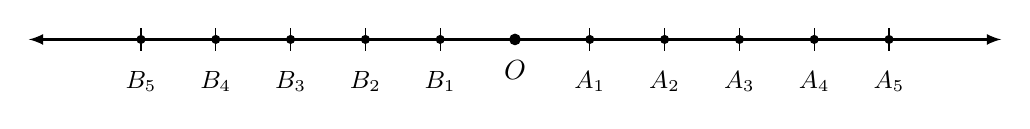
\begin{tikzpicture}[scale=0.95, >=latex]
  \draw[<->, thick] (-6.5, 0) -- (6.5, 0);
  \filldraw (0, 0) circle (2pt) node[below=4pt] {$O$};
  \foreach \x in {1, 2, 3, 4, 5} {
    \draw (\x, 0.15) -- (\x, -0.15) node[below=4pt] {\small $A_\x$};
    \filldraw (\x, 0) circle (1.5pt);
  }
  \foreach \x in {1, 2, 3, 4, 5} {
    \draw (-\x, 0.15) -- (-\x, -0.15) node[below=4pt] {\small $B_\x$};
    \filldraw (-\x, 0) circle (1.5pt);
  }
\end{tikzpicture}
\end{figure}

以 $A = A_1$ 為中心向右邊做弧交於 $A_2$，使 $A_1 A_2 = 1$，次第做去，對所有 $i \le n$ 均可取得 $A_i$ 點使 $A_{i-1} A_i = 1$。由數學歸納法知，向右可無限做下去；同理以 $B = B_1$ 為中心，向左邊次第做弧，得點 $B_2, B_3, \dots$，使得 $B_{i-1} B_i = 1$，由歸納法知向左亦可無限做下去。

由做法知每兩相鄰的弧點距離均為一單位，若規定向右為正，向左為負，則 $A_n$ 點與 $0$ 點距 $n$ 個單位，$B_n$ 與 $0$ 距 $-n$ 單位，這樣可以將整數與直線上的點做一一對應：
\begin{align*}
  \mathbb{Z} &= \{\dots, -n, \dots, -2, -1, 0, 1, 2, 3, \dots, n, \dots\} \\
  &\quad\quad \updownarrow \quad\quad\ \updownarrow \quad\ \updownarrow \ \updownarrow \ \updownarrow \ \updownarrow \ \updownarrow \ \updownarrow \quad\quad \updownarrow \\
  \text{點集} &= \{\dots, B_n, \dots, B_2, B_1, O, A_1, A_2, A_3, \dots, A_n, \dots\}
\end{align*}
如此整數的大小順序就是對應點在線上的左右相對位置，點集的元素稱為以 $0$ 為基準點的整數點，標上這些點的直線就是數軸的前身。以後要稱 $B_2$ 點為點 $(-2)$，$A_2$ 點為點 $2$。如此，$a < b$ 的充分必要條件為點 $a$ 在點 $b$ 左，或點 $b$ 在點 $a$ 右，用符號「點 $a <$ 點 $b$」表示。

比較兩數 $a$、$b$ 的大小，我們還可以說
\begin{itemize}
  \item[(i)] $a < b \iff a-b < 0$.
\end{itemize}
或
\begin{itemize}
  \item[(ii)] $a > b \iff a-b > 0$.
\end{itemize}
因為
\begin{align*}
  a < b &\iff b > a \iff \text{存在 } u > 0 \text{，使得 } b = a+u \\
  &\implies -(b-a) < 0 \implies a-b < 0.
\end{align*}
而
\begin{align*}
  a > b &\iff \text{存在 } u > 0 \text{，使得 } b+u = a \\
  &\implies u = a-b \implies a-b > 0.
\end{align*}

\noindent\textbf{註}：在正整數系中「沒有解」的意思是對任何正整數 $x$，$a+x=b$，亦即 $5+x=3$ 都不可能成立。（如果 $x$ 正，則 $5+x > 5 > 3$，所以 $5+x$ 永遠不會等於 $3$），因此我們知道 $5+x=3$ 在正整數系中沒有解，我們也可以看出 $3x=5$ 也不可能有一個正整數解。

\subsection*{習題 3-5}\label{sec:ex3-5}
\addcontentsline{toc}{subsection}{習題 3-5}

\begin{enumerate}[1., leftmargin=2em]
  \item 試證任何負整數皆小於任一正整數。
  \item 試比較下列各組數的大小：
  \begin{enumerate}[(1)]
    \item $100, \quad -50$.
    \item $-100, \quad 1$.
    \item $-2, \quad 20$.
    \item $-3, \quad -5$.
    \item $-1000, \quad -5$.
    \item $-1, \quad 1$.
  \end{enumerate}
\end{enumerate}

\subsubsection*{丙、整數系的性質}\label{subsec:int_properties}

\begin{enumerate}[(A)]
  \item \textbf{零的特性}：對任何整數 $a \in \mathbb{Z}$，恆有
  \begin{align*}
    a+0 &= 0+a = a \\
    a \cdot 0 &= 0 \cdot a = 0
  \end{align*}
  \item \textbf{負數和正數的關係}：
  \begin{align*}
    1+(-1) &= (-1)+1 = 0 \\
    2+(-2) &= (-2)+2 = 0 \\
    3+(-3) &= (-3)+3 = 0 \\
    n+(-n) &= (-n)+n = 0
  \end{align*}
  由於 $n+(-n) = (-n)+n = 0$ 是對的，我們很自然地可以記 $-(-n) = n$。
  \item \textbf{符號定則}：我們定義：
  \begin{align*}
    a \cdot (-b) &= (-b) \cdot a = -(ab) \\
    (-a) \cdot (-b) &= (-b) \cdot (-a) = a \cdot b
  \end{align*}
  （亦即正負（或負正）得負，負負得正！）。
  \item \textbf{整數系的基本性質}：對於「加」、「乘」整數滿足下列性質：
  \begin{enumerate}[(i)]
    \item $(a+b)+c = a+(b+c), \quad (a \cdot b) \cdot c = a \cdot (b \cdot c)$ 〔結合律〕
    \item $a+b = b+a, \quad a \cdot b = b \cdot a$ 〔交換律〕
    \item $a+0 = 0+a = a, \quad a \cdot 0 = 0 \cdot a = 0$ 〔零的特性〕
    \item $a \cdot (b+c) = a \cdot b + a \cdot c$ 〔分配律〕
    \item 對於任給 $a, b \in \mathbb{Z}$，$a+x=b$ 在 $\mathbb{Z}$ 中恆有解，〔加法可逆性〕\\
    （這個解就是 $b+(-a)$，一般簡寫為 $b-a$。）
    \item 如果 $c \neq 0$，$a \cdot c = b \cdot c$，則 $a = b$。〔乘法對消律〕
    \item 對於任意二整數 $a, b$ 下面的三個關係有一個，只有一個成立：
    \begin{equation*}
      (1)\ a < b, \qquad (2)\ a = b, \qquad (3)\ a > b.
    \end{equation*}
  \end{enumerate}
\end{enumerate}

\noindent{\textbf{【例 1】}}說明 $a(b-c) = ab - ac$。

\noindent{\textbf{【證明】}}
\begin{align*}
  a(b-c) &= a[b+(-c)] \\
  &= ab + a \cdot (-c) \\
  &= ab + (-ac) \\
  &= ab - ac.
\end{align*}
故得證。

\medskip
\noindent{\textbf{【例 2】}}$a \cdot 0 = 0$ 之說明

\begin{enumerate}[1.]
  \item $a \cdot 0 = a \cdot (1-1) = a \cdot 1 - a \cdot 1 = a - a = 0$。（$1-1=0$，分配律，$\because a \cdot 1 = a$）
  \item $a \cdot 0 = a \cdot (0+0) = a \cdot 0 + a \cdot 0$。（$0+0=0$，分配律）\\
  即 $0 + a \cdot 0 = a \cdot 0 + a \cdot 0 \implies 0 = a \cdot 0$。（對消律）
\end{enumerate}
故得證。

\medskip
我們已經證過對於自然數 $a, b, c$ 如果 $a > b$，那麼 $a \cdot c > b \cdot c$；但對整數來說，如果 $c < 0$，我們卻有 $a \cdot c < b \cdot c$。

\medskip
\noindent{\textbf{【例 3】}}如果 $a, b$ 是負數，而且 $a > b$，那麼當 $k$ 是正偶數時，$a^k < b^k$，而當 $k$ 是正奇數時，$a^k > b^k$，試證之。

設 $0 > a > b$。
\begin{enumerate}[(i)]
  \item 如果 $k$ 是正偶數，那麼 $a^k < b^k$。\\
  \textbf{證明}：令 $k = 2m$。
  \begin{align*}
    0 > a > b &\implies 0 < -a < -b \implies (-a)^2 < (-b)^2 \implies a^2 < b^2 \\
    &\implies (a^2)^m < (b^2)^m \implies a^{2m} < b^{2m} \implies a^k < b^k.
  \end{align*}
  \item 如果 $k$ 是正奇數時，那麼 $a^k > b^k$。\\
  \textbf{證明}：令 $k = 2m+1$。\\
  由 (i) 知 $a^{2m} < b^{2m}$。因 $0 > a > b$，所以 $a^{2m+1} > b^{2m+1}$，即 $a^k > b^k$。
\end{enumerate}

\subsection*{習題 3-6}\label{sec:ex3-6}
\addcontentsline{toc}{subsection}{習題 3-6}

\begin{enumerate}[1., leftmargin=2em]
  \item 由例 2 我們可以看出正整數的性質 XII 對於整數不成立，試分別討論各種情形，寫出他們的規則。
  \item 正整數性質 XII' 在整數情形下，也不成立，請舉例說明各種可能的情形。
  \item 如果 $a$ 是正數，$b$ 是負數，我們當然有 $a > b$，請討論這時 $a^k$ 與 $b^k$ 的大小關係（$k \in \mathbb{N}$）。
\end{enumerate}

\subsection{有理數系}\label{sec:3-4}

有理數就是比數，或稱分數。

\subsubsection*{甲、分數（有理數）}\label{subsec:fractions}

\begin{enumerate}[(i)]
  \item \textbf{分數的產生}：如 \ref{sec:3-3} 所說，下列方程式
  \begin{equation*}
    b \cdot x = a, \quad (b \neq 0)
  \end{equation*}
  在整數系中不一定有解，為了要使上式有解，我們將 $\mathbb{Z}$ 再加以擴張，同學們都知道這個擴張方法就是引入「分數」，一個分數就是形如 $\frac{a}{b}$（$a, b \in \mathbb{Z}, b \neq 0$）而滿足方程式 $bx=a$ 的數，換句話說，$b\left(\frac{a}{b}\right) = a$。

  譬如：
  \begin{itemize}
    \item $2 \cdot \left(\frac{1}{2}\right) = 1$，$\frac{1}{2}$ 為 $2x=1$ 之解。
    \item $5 \cdot \left(\frac{3}{5}\right) = 3$，$\frac{3}{5}$ 為 $5x=3$ 之解。
    \item $3 \cdot \left(\frac{5}{3}\right) = 5$，$\frac{5}{3}$ 為 $3x=5$ 之解。
    \item $(-3) \cdot \left(\frac{7}{-3}\right) = 7$，$\frac{7}{-3}$ 為 $-3x=7$ 之解。
    \item $(-6) \cdot \left(-\frac{5}{6}\right) = 5$，$-\frac{5}{6}$ 為 $-6x=5$ 之解。
  \end{itemize}
  所有的有理數所成的集合，用符號 $\mathbb{Q}$ 表之：
  \begin{equation*}
    \mathbb{Q} = \left\{\frac{a}{b} \;\middle|\; a, b \in \mathbb{Z}, \; b \neq 0\right\}.
  \end{equation*}
  由於 $1 \cdot a = a$，所以在有理數系中，我們也可以把 $a$ 看成 $\frac{a}{1}$ 的另一寫法，用這種辦法，整數便被看成分數的一種特例，換句話說，$\mathbb{Q} \supset \mathbb{Z}$。

  當 $a=1$，滿足方程式 $bx=1$ 的數，寫成 $\frac{1}{b}$，我們有 $b \cdot \left(\frac{1}{b}\right) = 1$。而稱 $\frac{1}{b}$ 為 $b$ 的乘法反元素。顯然，$\mathbb{Z}$ 中的元素除 $\pm 1$ 以外，均無乘法反元素，而 $\mathbb{Q}$ 中除了零以外，均有乘法反元素。

  \item \textbf{分數的表法}：\\
  當 $c \neq 0$ 時，由乘法的對消律可知
  \begin{align*}
    b \cdot x = a &\iff c(bx) = c \cdot (b \cdot x) = c \cdot a \\
    &\iff (cb)x = ca \\
    &\iff x = \frac{ca}{cb} = \frac{a}{b}
  \end{align*}
  所以分數 $\frac{a}{b}$ 亦即 $\frac{ca}{cb}$ 和 $\frac{a}{b}$ 是同一分數的兩種表法，由 $\frac{ca}{cb}$ 化成 $\frac{a}{b}$ 叫做\textbf{約分}；由 $\frac{a}{b}$ 化成 $\frac{ca}{cb}$ 叫做\textbf{擴分}。

  有理數的另一種表示法便是「小數」。關於小數的觀念，同學們在小學及國中階段都已十分熟悉，任何一個有理數皆可化為小數（有限或循環），反之，任一有限或循環小數，皆可化為一有理數，關於這一點，我們以後還要再講到。

  \item \textbf{分數的運算}：\\
  在小學中，同學們即已熟悉分數的加法與乘法，它們的定義可以用式子表之如下：
  \begin{align*}
    \frac{a}{b} + \frac{c}{d} &= \frac{ad}{bd} + \frac{bc}{bd} = \frac{ad+bc}{bd} \\
    \left(\frac{a}{b}\right) \cdot \left(\frac{c}{d}\right) &= \frac{ac}{bd}
  \end{align*}
  我們定義有理數的加法與乘法，當然希望它滿足數系的基本性質，如結合律、交換律、分配律等，在這個要求下，就不得不像上面這樣定義，我們可以略為解釋一下。

  由 $\frac{a}{b}$ 和 $\frac{c}{d}$ 的定義有：
  \begin{equation*}
    b\left(\frac{a}{b}\right) = a, \quad d\left(\frac{c}{d}\right) = c.
  \end{equation*}
  \begin{align*}
    (bd)\left[\frac{a}{b} + \frac{c}{d}\right] &= (bd)\left(\frac{a}{b}\right) + (bd)\left(\frac{c}{d}\right) \\
    &= d\left[b\left(\frac{a}{b}\right)\right] + b\left[d\left(\frac{c}{d}\right)\right] \\
    &= da + bc = ad + bc.
  \end{align*}
  由分數的定義，得 $\frac{a}{b} + \frac{c}{d} = \frac{ad+bc}{bd}$。

  同理，
  \begin{equation*}
    (bd)\left[\left(\frac{a}{b}\right)\left(\frac{c}{d}\right)\right] = \left[b\left(\frac{a}{b}\right)\right]\left[d\left(\frac{c}{d}\right)\right] = ac.
  \end{equation*}
  故 $\left(\frac{a}{b}\right)\left(\frac{c}{d}\right) = \frac{ac}{bd}$。

  \item \textbf{有理數系的基本性質}：\\
  對任意有理數 $r, s, t \in \mathbb{Q}$：
  \begin{align*}
    r+0 &= 0+r = r, && \text{〔零的特性〕} \\
    r \cdot 1 &= 1 \cdot r = r, && \text{〔1 的特性〕} \\
    r \cdot 0 &= 0 \cdot r = 0
  \end{align*}
  對於任何 $r$ 存在一唯一的 $-r$，使得 $r+(-r) = 0$。〔加法可逆性〕\\
  對於任給 $r \neq 0$，存在唯一的 $\frac{1}{r}$（稱為 $r$ 的倒數），使得 $r \cdot \left(\frac{1}{r}\right) = 1$。〔乘法可逆性〕\\
  $r \cdot (s+t) = r \cdot s + r \cdot t$。〔分配律〕\\
  （加法與乘法之結合律、交換律在此亦皆成立）。

  \item \textbf{次序關係}：\\
  像整數一樣，有理數是可以比較大小的，而且對於任給兩數 $r$、$s \in \mathbb{Q}$，下列三情形：$r < s, r = s, r > s$ 只有一種成立。

  我們在前面已經說明了怎樣比較兩個整數的大小。在這裏，我們再說明一下怎樣比較兩個有理數的大小，因為有理數都可以擴分，我們可以把任何兩個有理數分別擴分，使得它們的分母為相等的正整數，這時，我們便可以比較它們的分子，分子大的分數較大。

  例如：$-\frac{3}{8}$ 和 $-\frac{1}{2} = -\frac{4}{8}$，因為 $-3 > -4$，故 $-\frac{3}{8} > -\frac{1}{2}$。
\end{enumerate}

\subsection*{習題 3-7}\label{sec:ex3-7}
\addcontentsline{toc}{subsection}{習題 3-7}

\begin{enumerate}[1., leftmargin=2em]
  \item 試算出下列各式的結果，並分別比較它們的大小。
  \begin{enumerate}[(i)]
    \item $\left(-\frac{1}{2}\right) + \frac{2}{3} - \left(-\frac{3}{4}\right)$ 和 $\left(-\frac{1}{2}\right)\left(\frac{2}{3}\right) - \left(-\frac{3}{4}\right)\left(-\frac{1}{2}\right)$。
    \item $\left(\frac{2}{3}\right)\left[\frac{3}{4} + \frac{5}{6} - \left(-\frac{1}{2}\right)\right] \div \left(\frac{4}{12}\right)$ 和 $\left[\left(-\frac{3}{8}\right)\left(-\frac{2}{9}\right) + \frac{1}{6}\right] \div (-6)$。
  \end{enumerate}
  \item 算出下列各組數的算術平均數：
  \begin{enumerate}[(i)]
    \item $25, \quad -77, \quad 27$。
    \item $\frac{5}{9}, \quad \frac{1}{10}, \quad \frac{7}{2}, \quad \frac{17}{9}, \quad \frac{2}{3}, \quad \frac{1}{2}$。
  \end{enumerate}
  \item 試將下列各數大小關係排成一列：
  \begin{equation*}
    -\frac{3}{4}, \quad \frac{5}{8}, \quad -1, \quad -\frac{7}{6}, \quad -1.12, \quad 1.24.
  \end{equation*}
  \item 設 $a$、$b$ 為任意兩個有理數，則永遠可在 $a$、$b$ 之間找到第三個有理數 $c$。
  \item 試證對於 $a, b \in \mathbb{Q}$
  \begin{enumerate}[(i)]
    \item $a < b \iff -a > -b$。
    \item $\frac{b}{a} > 0 \iff ab > 0$。
    \item $\frac{a}{b} < \frac{c}{d}, \quad bd > 0 \implies ad < bc$。
    \item $\frac{a}{b} < \frac{c}{d}, \quad bd < 0 \implies ad > bc$。
  \end{enumerate}
  \item 設 $a, b, c$ 為三有理數，且 $a+b+c=0$。\\
  試證 $a\left(\frac{1}{b} + \frac{1}{c}\right) + b\left(\frac{1}{c} + \frac{1}{a}\right) + c\left(\frac{1}{a} + \frac{1}{b}\right) = -3$。
  \item 設 $a, b, c, d$ 為四正有理數，且 $\frac{a}{b} < \frac{c}{d}$。\\
  試證 $\frac{a}{b} < \frac{a+c}{b+d} < \frac{c}{d}$。
  \item 計算 $0.2+0.22+0.222+\dots$（$n$ 項的和）。
  \item $5.5+55.55+555.555+\dots$（$n$ 項的和）。\\
  （提示：利用上題及習題 3-4 第 8 題）
\end{enumerate}

\subsection{實數}\label{sec:3-5}

任意兩有理數間有第三個有理數（習題 3-7，第 4 題），而由歸納法可知兩有理數間其實有無數個有理數。

將這些數標到一條定了基準點的直線上，試問這些點能否把連接所給兩有理點的線段填滿？答案是：\textbf{不可以的}。不但如此，點 $a$ 與點 $b$ 間且有許多（也是無數個）空隙，我們將把這些空隙上的點所對應的量叫做\textbf{無理數}，而這些點又將稱為無理點，這樣一來，加進了無理點之後，原來兩點間就不再有空隙了，而且無理數是不能用分數形式來表示的。（否則……？）

無理數的產生除了可以從以上填充空隙的需要來看，也可如整數及分數的產生是為得到方程式之解（\ref{sec:3-3}, \ref{sec:3-4}）的需要來看。即 $\sqrt{2}$、$\sqrt{3}$、$\sqrt{5}$……不是有理數，它們是為滿足方程式 $x^2=2, x^2=3, x^2=5, \dots$ 而加入的。

有理數集與無理數集做成\textbf{實數集}。有關實數的性質要到下一冊再講。

對任意實數 $a$，定義
\begin{align*}
  |a| &= a \quad (\text{當 } a \ge 0) \\
  &= -a \quad (\text{當 } a < 0)
\end{align*}
稱為實數 $a$ 的\textbf{絕對值}。

\subsection*{習題 3-8}\label{sec:ex3-8}
\addcontentsline{toc}{subsection}{習題 3-8}

試利用上面定義，證明
\begin{enumerate}[(i), leftmargin=2.5em]
  \item $\sqrt{a^2} = |a|$.
  \item $|ab| = |a||b|$.
  \item $\left|\frac{a}{b}\right| = \frac{|a|}{|b|}$.
  \item $-|a| \le a \le |a|$.
  \item $\delta > 0, \quad |x| < \delta \iff -\delta < x < \delta$.
  \item $\delta > 0, \quad |x| > \delta \iff x > \delta \text{ 或 } x < -\delta$.
  \item $|a+b| \le |a| + |b|$.
  \item $|a-b| \le |a| + |b|$.
  \item $\big||a| - |b|\big| \le |a+b|$.
  \item $\big||a| - |b|\big| \le |a-b|$.
\end{enumerate}
